\chapter{Introduction}
\label{ch.intro}

% Context
% Historical background
% Frequency barrier
	For some years, it was common to increase the frequency of processors
	to improve their processing power.
	However, as a side effect, the temperature rise was much higher than the
	performance, making this practice prohibitive.
	Alternatively, the constant improvement of semiconductor technology helped
	to mitigate the impact of this problem, allowing the industry to build
	more powerful processors with the same frequency.
	Therefore, knowing the frequency barrier and the imminent end of Moore's Law~\cite{moore:1965},
	the academy and industry began to research and invest in alternatives
	to keep increasing the processing power of computer systems.

% Improves architectural parts
	Such researches have led to a wide diversity of trade-offs in modern architectures.
	For instance, different types of instruction sets, instruction parallelism,
	out-of-order processing techniques, detour prediction techniques, and various
	memory hierarchies were some of the key techniques proposed to improve the
	performance of a single core.
	Then, the performance of computer systems has been improved even further by
	increasing the number of processing cores in a single die.
	These architectures, called \textit{multicores}, allowed the continuous
	rise of the computing performance.

% + Rephrasing by Pedro {
	The ever-increasing number of transistors and cores in a chip quickly lead
	to the advent of \manycores.
	Notwithstanding, the line between \textit{multicores} and \manycores is very tenuous.
	Some researchers argue that the in latter architectures, \todo{não entendi}{having a core go to down
	it will not significantly impact the performance of the platform}.
	\todo{estranho... qual fonte da classificação?}{A system is classified as \manycore when there is a need for distributed memory and on-chip networking}.
% + }

	\begin{figure}[h]
		\centering
		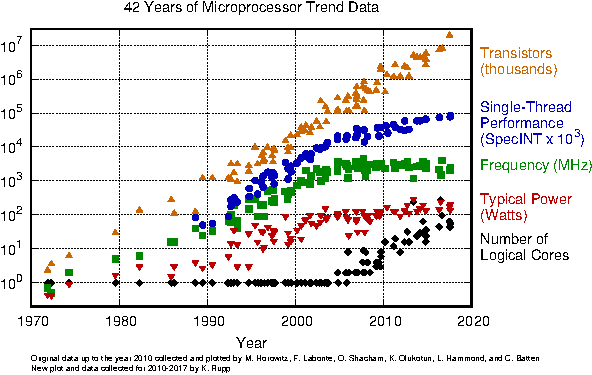
\includegraphics[width=.85\textwidth]{images/42-years-processor-trend.pdf}

		\caption{
			42 years of Multiprocessor Trend Data~\cite{url:microprocessor-trend-data}.
		}\par
		\label{fig.microprocessor-data}
	\end{figure}

% From multicore to manycores and Manycores characteristics
	Yet another classification is based on the ratio between processing power (\flops)
	and power consumption (\watts) of a manycore, as shown in Figure \ref{fig.microprocessor-data}.
	For instance, to achieve \exascale (10$^{18}$ \flops), the US Department of Defense
	issued a report stipulating the energy efficiency of a supercomputer should be
	around 50 GFLOPS/W~\cite{darpa:exascale}.
	Recently, a new class of parallel processors, called \textit{lightweight} \manycores,
	has emerged to provide high parallelism with low power consumption.
	These processors own the following characteristics:

	\begin{itemize}
		\item They integrate thousands of low-power cores in a single die organized in clusters;
		\item They are designed to cope with \mimd workloads;
		\item They rely on a high-bandwidth \noc for fast and reliable message-passing communication;
		\item They present constrained memory systems; and
		\item They frequently feature a heterogeneous configuration.
	\end{itemize}

	Some industry-successful examples of \textit{lightweight} \manycores are
	the \mppa~\cite{DeDinechin2013-1};
	the \epiphany~\cite{olofsson2014}; and
	the \taihulight~\cite{zheng2015}.

% Motivation
	Jointly with further performance scalability and energy efficiency, manycores brought a new
	set of challenges in software development coming from their architectural particularities.
	Precisely, these particularities introduce the following difficulties:
	\begin{itemize}
		\item \textbf{Hybrid programming model:} due to the parallel and distributed nature of
			the architecture, engineers are frequently required to adopt a message-passing
			programming model to deal with the presence of rich \nocs~\cite{kelly2013} that
			interconnects clusters and a shared-memory model inside the cluster.
		\item \textbf{Missing hardware support for cache coherency:} to reduce power consumption,
			theses processors do not feature cache coherency, which in turn forces programmers to
			handle it explicitly in software level and frequently calls out for a redesign in their
			applications~\cite{francesquini2015};
		\item \textbf{Constrained memory system:} the frequent presence of multiple physical
			address spaces and small local memories require data tiling and prefetching to be
			handled by the software~\cite{Castro2016};
		\item \textbf{Heterogeneous configuration:} the different programmable components on
			\textit{lightweight} \manycores turns the actual deployment of applications in a
			complex task~\cite{barbalace2015}.
	\end{itemize}

% Challenges and Problem Definition
	Part of these challenges derives from existing runtimes and \oses.
% Primeiro as dificuldades que não são superadas apenas com um runtime.
	On the one hand, runtimes do not hide the characteristics of hardware making
	software development more challenging and nonportable, \eg do not allow
	direct access to non-local data, nor the manipulation of them in a transparent way.
% Concluir com a idea de que runtimes não proporcionam resource sharing and multiplexing.
	Thus, fundamental \os mechanisms, such as core multiplexing, core partitioning,
	and process and data migration, may not be addressed.
% E, então, mencionar esforços em designs alternativos.
	On the one hand, the complicated portability and scalability of traditional \oses with a
	monolithic kernels, which were designed to homogeneous hardwares, is leading to alternative
	\os designs~\cite{Baumann2009, kluge2014, nightingale2009, rhoden2011}.

% Goals and Contributions
	We believe that \oses for the next-generation of \textit{lightweight} \manycores must be
	redesigned from scratch to cope with their tight architectural constraints.
	Based on this idea, a new fully-featured distributed \os based on a \multikernel approach~\cite{Baumann2009}
	is being proposed~\cite{penna2017-1,penna2017-2,penna2019}.
	The \nanvix \multikernel features a generic and flexible \hal for \textit{lightweight} \manycores that
	addresses the key issues encountered in the development for these processors.
	On top of the \nanvix \hal, we are simultaneously designing and implementing a \microkernel
	that provides bare bones system abstractions for each cluster.

\section{Goals}
\label{sec.goals}

	Based on the aforementioned motivations, the primary and specific goals of this work are detailed next.

\subsection{General Goals}
\label{sec.goals.general}

	The foremost goal of this undergraduate dissertation is to propose a \textit{Inter-Cluster Communication Module}
	to the \nanvix \hal and port it to the \mppa manycore processor~\cite{DeDinechin2013-1}.
	This module will expose the essential abstractions that permit upper layers to create more
	sophisticated communication services.
	Using this module, we also propose \textit{Inter-Cluster Communication Services} to the \nanvix Microkernel.
	This work will be done in collaboration with Pedro H. Penna, who is a Ph.D. student at the
	University of Grenoble Alpes, the main developer of Nanvix and the co-advisor of this work.

\subsection{Specific Goals}
\label{sec.goals.specific}

	\begin{itemize}
		\item Propose interfaces to the Inter-Cluster Communication Module aiming
			the class of \textit{lightweight} \manycore processors;
		\item Implement the interfaces for the \textit{\mppa manycore processor};
		\item Define Communication Services and their strategies in the use of the Inter-Cluster
			Communication Module in the context of a microkernel-based \os;
		\item Implement the Communication Services for the \nanvix Microkernel;
		\item Analyze the performance of the proposed implementation using specific micro-benchmarks.
	\end{itemize}

\section{Organization Of The Work}
\label{sec.organization}

	This will be written last.